\chapter{SYSTEM DESIGN} \label{c4}
\justifying

\section{Overview}

This chapter presents the system architecture and component design for the Sign Language Interpreter.

\vspace{1em}
\section{System Architecture}

The system follows a layered architecture: the User Interface Layer provides the Streamlit web interface with live webcam display, prediction output, and controls; the Application Layer orchestrates the inference pipeline and text buffering; the Processing Layer handles video capture, ML inference, and text-to-speech; and the Detection Layer uses MediaPipe for landmark extraction.
% System Architecture Diagram
\begin{figure}[H]
\centering
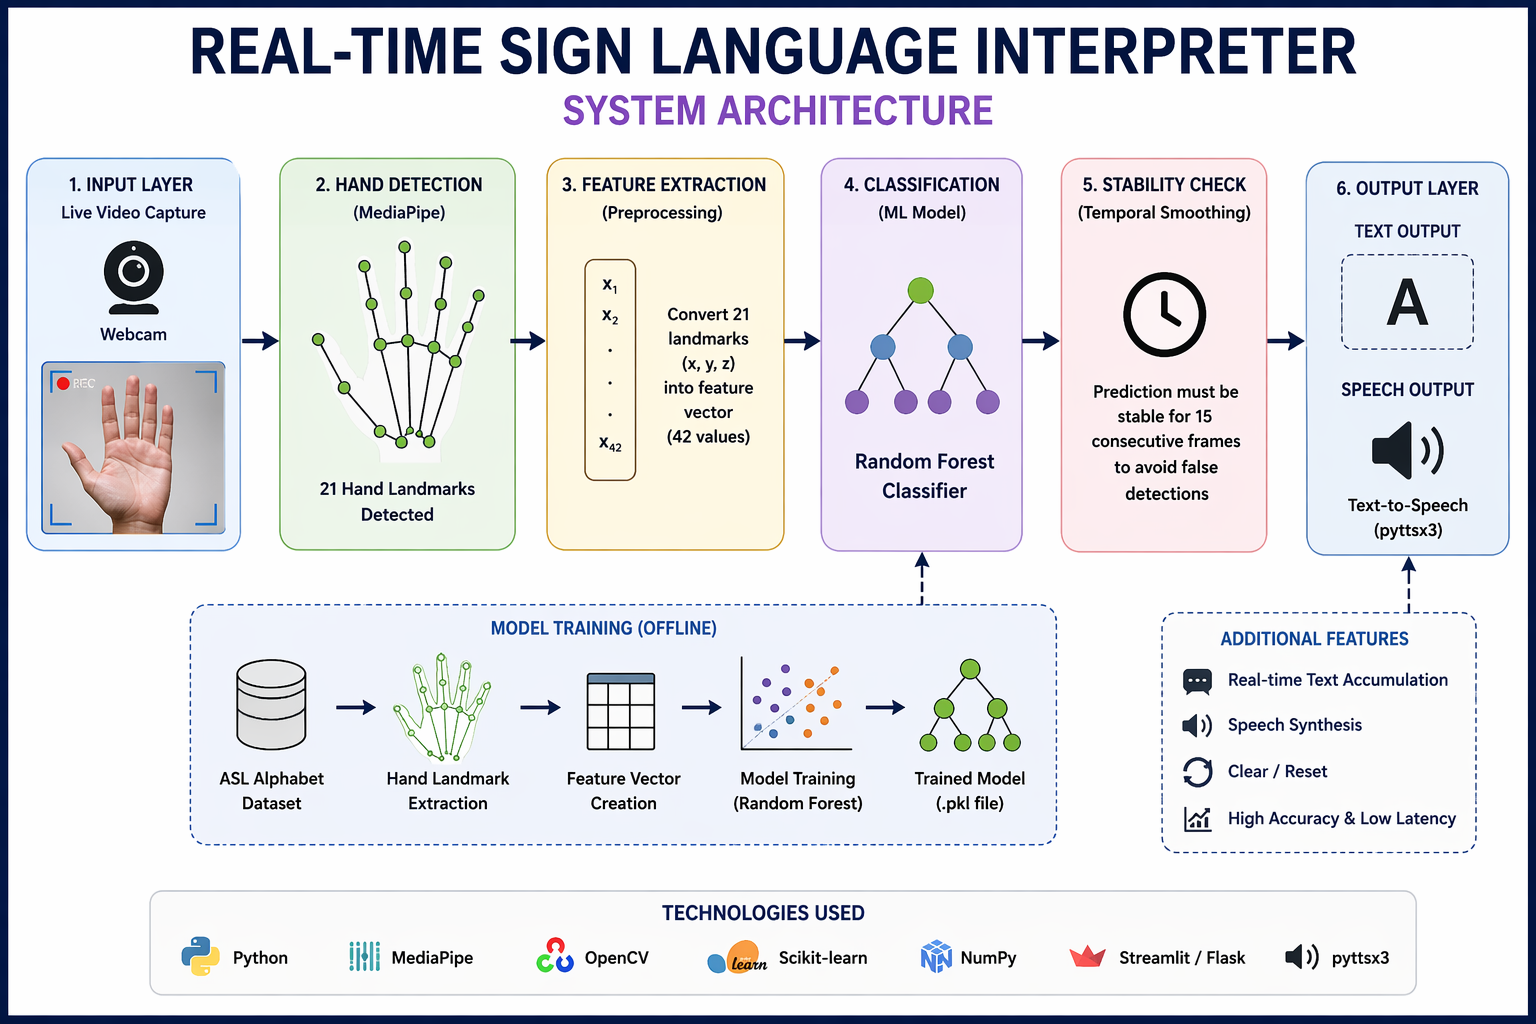
\includegraphics[width=0.8\textwidth]{images/arc.png}
\caption{System Architecture}
\label{c4:fig1}
\end{figure}

\vspace{1em}
\section{Component Design}

The system comprises seven components operating in sequence. Video Capture acquires frames at 640x480, applies horizontal flip and BGR-to-RGB conversion. Hand Detection uses MediaPipe to extract 21 landmarks per hand with detection confidence threshold 0.7. Feature Extraction normalizes all landmarks relative to the wrist (landmark 0), discarding the z-coordinate to produce a 42-dimensional feature vector. Classification uses a trained Random Forest (200 trees, max depth 15) to predict letters with confidence scores. Stability Checker requires 15 consecutive frames with confidence above 0.85 before accepting a prediction. Text Processing buffers letters into words, with special gestures for space and delete. Output Module displays results and generates speech via TTS.

The 21 MediaPipe landmarks include the wrist (index 0), thumb (1-4), index (5-8), middle (9-12), ring (13-16), and pinky (17-20).
% 21 MediaPipe Diagram
\begin{figure}[H]
\centering
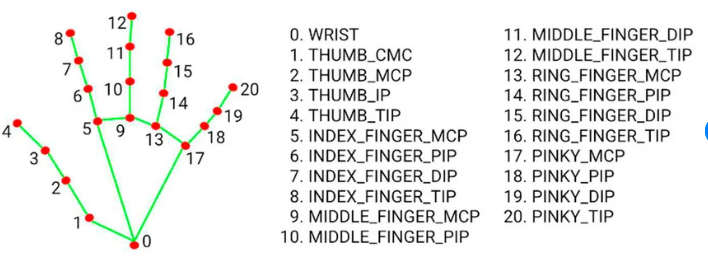
\includegraphics[width=0.8\textwidth]{images/21pi.png}
\caption{21 MediaPipe Landmarks}
\label{c4:fig2}
\end{figure}

\vspace{1em}
\section{Data Flow}

The inference loop: capture frame, detect hand, extract features, classify, check stability, update buffer, display, repeat.
% Data flow diagram
\begin{figure}[H]
\centering
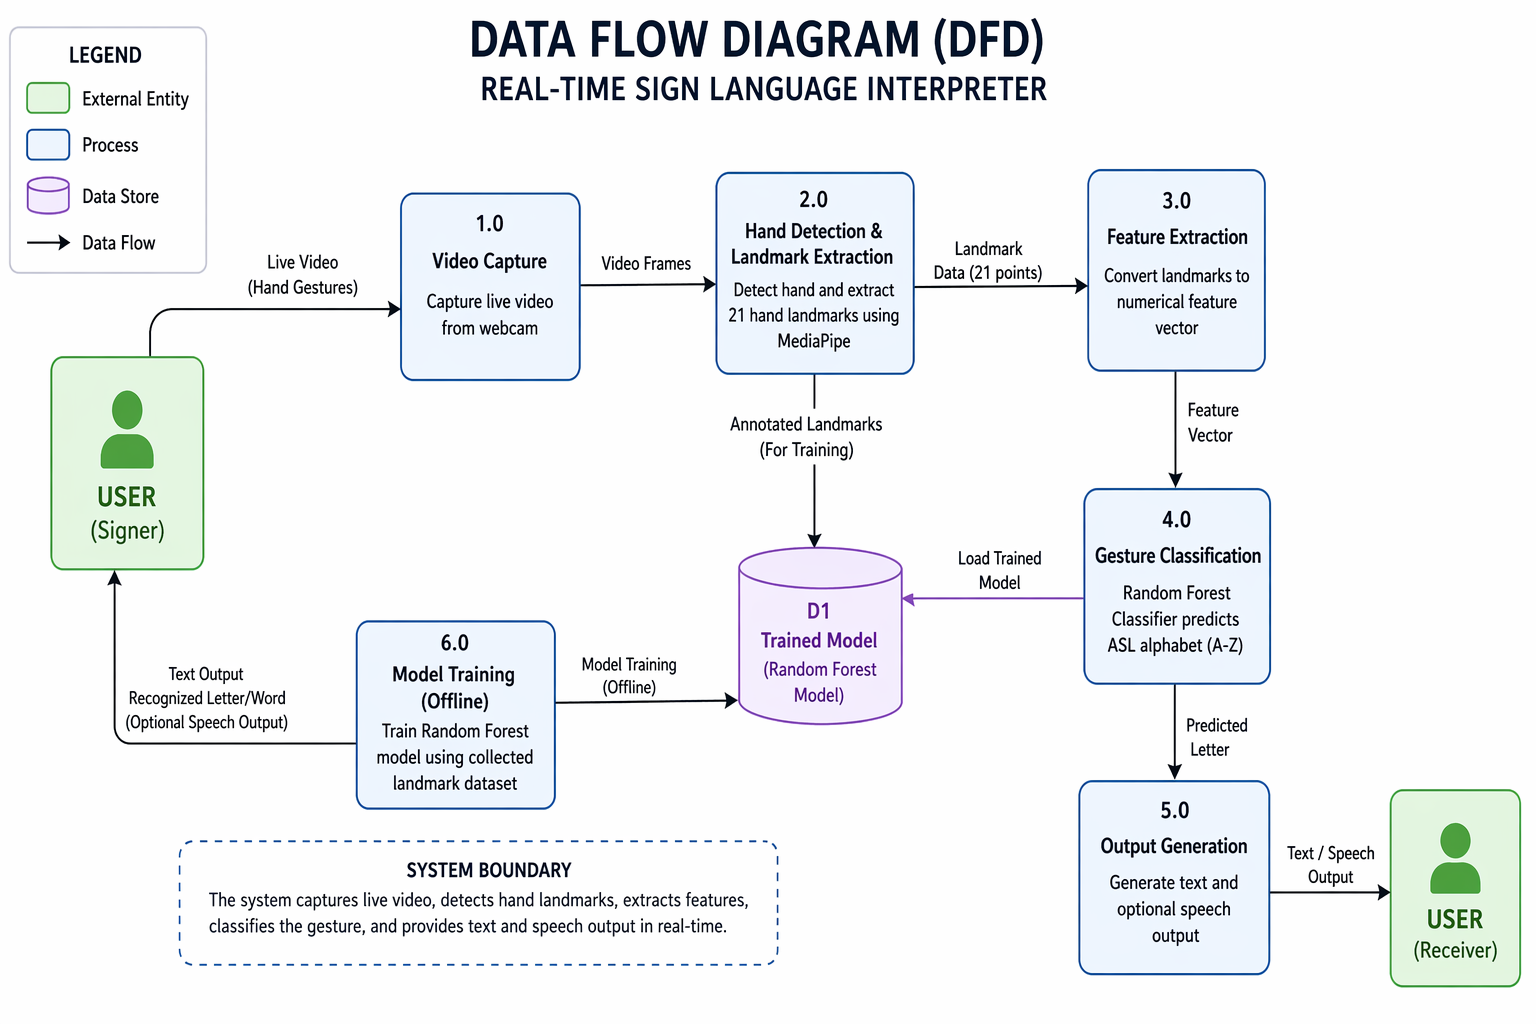
\includegraphics[width=0.8\textwidth]{images/data.png}
\caption{Data Flow}
\label{c4:fig3}
\end{figure}

\vspace{1em}
\section{State Machine}

The system operates in states: IDLE (waiting for hand), DETECTION (extracting landmarks), PREDICTION (classifying gesture), STABILITY (counting frames), CONFIRMED (adding to buffer), WORD COMPLETE (triggering TTS).

\vspace{1em}
\section{Summary}

This chapter presented the layered architecture, seven sequential components, data flow, and state machine providing a blueprint for implementation.